% !TeX program = pdfLaTeX
\documentclass[12pt]{article}
\usepackage{amsmath}
\usepackage{graphicx,psfrag,epsf}
\usepackage{enumerate}
\usepackage{natbib}
\usepackage{textcomp}
\usepackage[hyphens]{url} % not crucial - just used below for the URL
\usepackage{hyperref}
\providecommand{\tightlist}{%
  \setlength{\itemsep}{0pt}\setlength{\parskip}{0pt}}

%\pdfminorversion=4
% NOTE: To produce blinded version, replace "0" with "1" below.
\newcommand{\blind}{0}

% DON'T change margins - should be 1 inch all around.
\addtolength{\oddsidemargin}{-.5in}%
\addtolength{\evensidemargin}{-.5in}%
\addtolength{\textwidth}{1in}%
\addtolength{\textheight}{1.3in}%
\addtolength{\topmargin}{-.8in}%

%% load any required packages here



\usepackage{amsmath}
\usepackage{amsfonts}
\usepackage{booktabs}
\usepackage{makecell}
\usepackage[usenames, dvipsnames]{color}
\usepackage{multirow}
\usepackage{comment}
\usepackage{booktabs}
\usepackage{longtable}
\usepackage{array}
\usepackage{wrapfig}
\usepackage{float}
\usepackage{colortbl}
\usepackage{pdflscape}
\usepackage{tabu}
\usepackage{threeparttable}
\usepackage{threeparttablex}
\usepackage[normalem]{ulem}
\usepackage{xcolor}
\newcommand{\beginsupplement}{\setcounter{table}{0} \renewcommand{\thetable}{S\arabic{table}}\setcounter{figure}{0} \renewcommand{\thefigure}{S\arabic{figure}}}

\begin{document}


\def\spacingset#1{\renewcommand{\baselinestretch}%
{#1}\small\normalsize} \spacingset{1}


%%%%%%%%%%%%%%%%%%%%%%%%%%%%%%%%%%%%%%%%%%%%%%%%%%%%%%%%%%%%%%%%%%%%%%%%%%%%%%

\if0\blind
{
  \title{\bf Descriptive Paper Title}

  \author{
        Mathew E. Hauer \thanks{Thanks y'all!} \\
    Department of Sociology, Florida State University\\
     and \\     Scientist 2 \\
    Department of Department, Random State University\\
      }
  \maketitle
} \fi

\if1\blind
{
  \bigskip
  \bigskip
  \bigskip
  \begin{center}
    {\LARGE\bf Descriptive Paper Title}
  \end{center}
  \medskip
} \fi

\bigskip
\begin{abstract}
Lorem Ipsum.
\end{abstract}

\noindent%
{\it Keywords:} keyword, keyword, keyword
\vfill

\newpage
\spacingset{1.45} % DON'T change the spacing!

\newpage

\hypertarget{introduction}{%
\section{Introduction}\label{introduction}}

This is an introduction. This is a citation
\citep{foxBackNoAnalogFuture2007}

You can also embed plots (\textbf{\autoref{fig-pressure}}), for example:

\begin{figure}
\centering
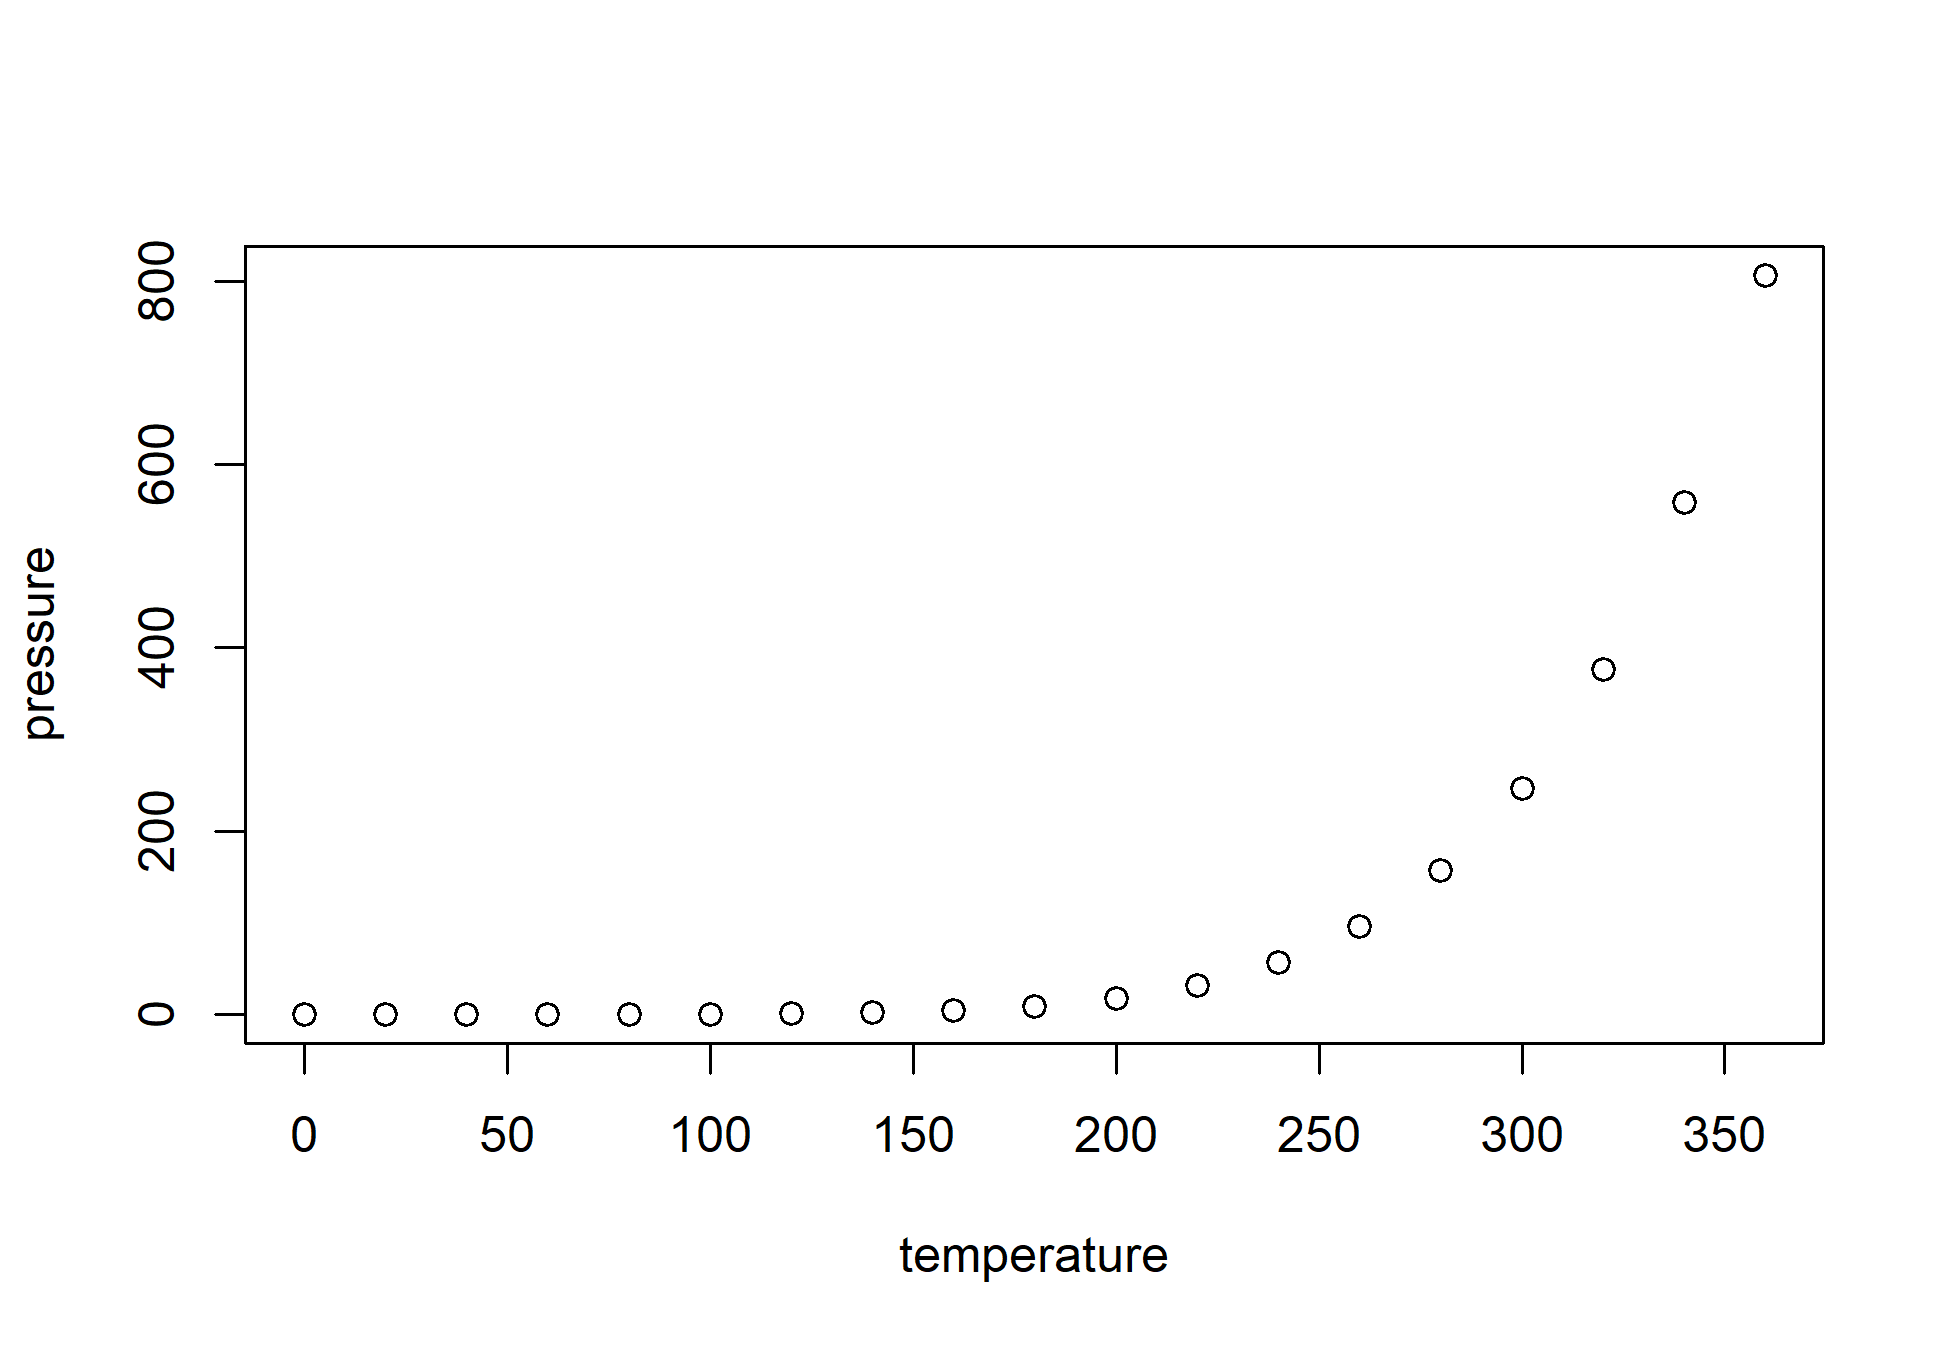
\includegraphics{manuscript_files/figure-latex/pressure-1.png}
\caption{\textbf{Title of the figure.} Solid dots show blah blah blah.
\label{fig-pressure}}
\end{figure}

And you can embed tables (\textbf{\autoref{error-table}}):

\begin{table}[t]

\caption{\label{tab:cars}\label{error-table}\textbf{Summary statistics for cars.} APE is the Description here.}
\centering
\resizebox{\linewidth}{!}{
\begin{tabular}{lll}
\toprule
  &     speed &      dist\\
\midrule
 & Min.   : 4.0 & Min.   :  2\\

 & 1st Qu.:12.0 & 1st Qu.: 26\\

 & Median :15.0 & Median : 36\\

 & Mean   :15.4 & Mean   : 43\\

 & 3rd Qu.:19.0 & 3rd Qu.: 56\\

\multirow{-6}{*}{\raggedright\arraybackslash } & Max.   :25.0 & Max.   :120\\
\bottomrule
\end{tabular}}
\end{table}

\newpage

\bibliographystyle{agsm}
\bibliography{mybibfile}

\end{document}
